\chapter{Fourier analysis on finite groups}
\label{chap-transforme-fourier-finite-group}
\chapteroverview{Fourier analysis represents a function by elementary components
adapted to the symmetries of its domain. On a finite abelian group, these
components are the characters, and all calculations involve finite sums.
This chapter constructs the Fourier transform, proves inversion and
orthogonality formulas, and explains why convolution becomes multiplication.}

The finite setting separates the algebra of Fourier analysis from questions
of convergence and regularity. It also provides the foundations of the fast
transforms developed later. We begin with cyclic groups, extend the theory to
finite abelian groups, and identify the obstruction in the noncommutative case.
For complementary accounts, see Serre~\cite{serre},
Warusfel~\cite{warusfel}, and Dym and McKean~\cite{dym}.

\section{Dual of a finite group}
\label{sect1-dual-group}
A function $f:G\to\CC$ can always be represented by its values. To exploit the
group structure, we instead seek elementary functions that respect
multiplication in $G$.

\subsection{Definitions}
\begin{defn}[Characters and the dual group]
\label{notation-0}\label{notation-1}
\index{Character!of an abelian group}\index{Dual!of a finite abelian group}
A \emph{linear character} of a finite group $G$ is a group homomorphism
$\chi:G\to\CC^*$. The set of these characters is denoted by $\wh G$ and is
called the \emph{dual group}. In the present chapter, ``character'' always means
linear character. Chapter~\ref{chap-linear-representations-finite-groups}
introduces the more general characters of linear representations.
\end{defn}
Pointwise multiplication makes $\wh G$ an abelian group:
\[
 (\chi_1\chi_2)(x)=\chi_1(x)\chi_2(x).
\]
Its identity is the constant character $1$, and the inverse of $\chi$ is
$x\mapsto\chi(x)^{-1}$.

\begin{prop}
\label{prop-pte-elem-car}
\label{notation-2}\label{notation-3}\label{notation-4}\label{notation-5}
If $|G|=n$, every character takes values in the group of $n$th roots of unity,
\[
 \UU_n=\{e^{2\pi\imath k/n}:0\leq k<n\}.
\]
Consequently, for every $g\in G$,
\[
 |\chi(g)|=1,\qquad
 \chi(g^{-1})=\chi(g)^{-1}=\ol{\chi(g)}.
\]
\end{prop}
\begin{proof}
Lagrange's theorem gives $g^n=1$. Applying $\chi$ yields
$\chi(g)^n=\chi(g^n)=1$.
\end{proof}

\begin{rem}
There are only finitely many maps $G\to\UU_n$, so $\wh G$ is finite.
Every linear character is constant on conjugacy classes, since
\begin{equation}
\label{eq-character-constant-class-conjug}
 \chi(h^{-1}gh)=\chi(h)^{-1}\chi(g)\chi(h)=\chi(g).
\end{equation}
\end{rem}

\begin{defn}[Functions on $G$]
\label{defn-space-function-g-in-c}
\label{notation-6}\label{notation-7}\label{notation-8}\label{notation-9}\label{notation-10}
\index{Space!of functions on a group}
Let $\CC[G]$ denote the complex vector space of functions $G\to\CC$.
We equip it with the normalized Hermitian inner product
\begin{equation}
\label{eq-defn-prod-herm-c-g-abelien}
 \dotp fg=\frac1{|G|}\sum_{x\in G}f(x)\ol{g(x)},
 \qquad \norm f_2^2=\dotp ff.
\end{equation}
The inner product is linear in its first argument.
\end{defn}

\begin{rem}
\label{notation-11}\index{Translation}
This inner product is the finite analogue of
$\dotp fg=\int_{\RR}f(x)\ol{g(x)}\,\d x$ on $L^2(\RR)$.
Both are translation invariant. For example, setting
$T_yf(x)=f(xy)$ gives
$\dotp{T_yf}{T_yg}=\dotp fg$ because $x\mapsto xy$ permutes $G$.
\end{rem}

\begin{prop}
\label{prop-base-c-g}
\index{Basis!Dirac}
The functions $(\delta_g)_{g\in G}$, defined by
\begin{equation}
\label{eq-defn-delta-function-g}
 \delta_g(h)=\begin{cases}1&h=g,\\0&h\neq g,\end{cases}
\end{equation}
form a basis of $\CC[G]$. In particular, $\dim_{\CC}\CC[G]=|G|$.
\end{prop}
\begin{proof}
Evaluating a linear combination at each $h\in G$ proves linear independence.
The identity
\begin{equation}
\label{eq-decomposition-c-g-dirac-abelien}
 f=\sum_{g\in G}f(g)\delta_g
\end{equation}
proves that the family spans the space. With the normalization
\eqref{eq-defn-prod-herm-c-g-abelien}, these basis vectors are orthogonal but
have squared norm $1/|G|$. Thus $(\sqrt{|G|}\,\delta_g)_{g\in G}$ is orthonormal.
\end{proof}
The injection $g\mapsto\delta_g$ will later give the group algebra its
multiplication. For Fourier analysis, we seek a different basis: one that
respects translations and simplifies convolution.

\subsection{Dual of a cyclic group}
\label{sect1-dual-cyclic-group}
Cyclic groups are both the simplest examples and the domains of the
one-dimensional discrete transforms used in signal processing.

\begin{prop}[The cyclic case]
\label{prop-cyclic-case}\label{notation-12}\label{notation-13}
\index{Group!cyclic}
Let $G=\langle g_0\rangle$ have order $n$, and set $\omega=e^{2\pi\imath/n}$.
Its characters are exactly
\[
 \chi_j(g_0^k)=\omega^{jk}=e^{2\pi\imath jk/n},
 \qquad 0\leq j<n.
\]
The map $j\mapsto\chi_j$ is an isomorphism $\ZZ/n\ZZ\to\wh G$.
\end{prop}
\begin{proof}
A character is determined by its value at $g_0$, which must be an $n$th root
of unity. Each choice $\chi(g_0)=\omega^j$ defines a character, since the
formula is unchanged when $k$ is replaced by $k+n$. The resulting characters
are distinct and satisfy $\chi_j\chi_k=\chi_{j+k}$, with indices modulo $n$.
\end{proof}
Figure~\ref{fig-cyclic-characters} shows $\chi_j$ for $j=0,1,2,3$ on
$\ZZ/12\ZZ$. Their real and imaginary parts sample
$\cos(2\pi jx/12)$ and $\sin(2\pi jx/12)$ at integer values of $x$.

\begin{figure}[tbp]
\centering
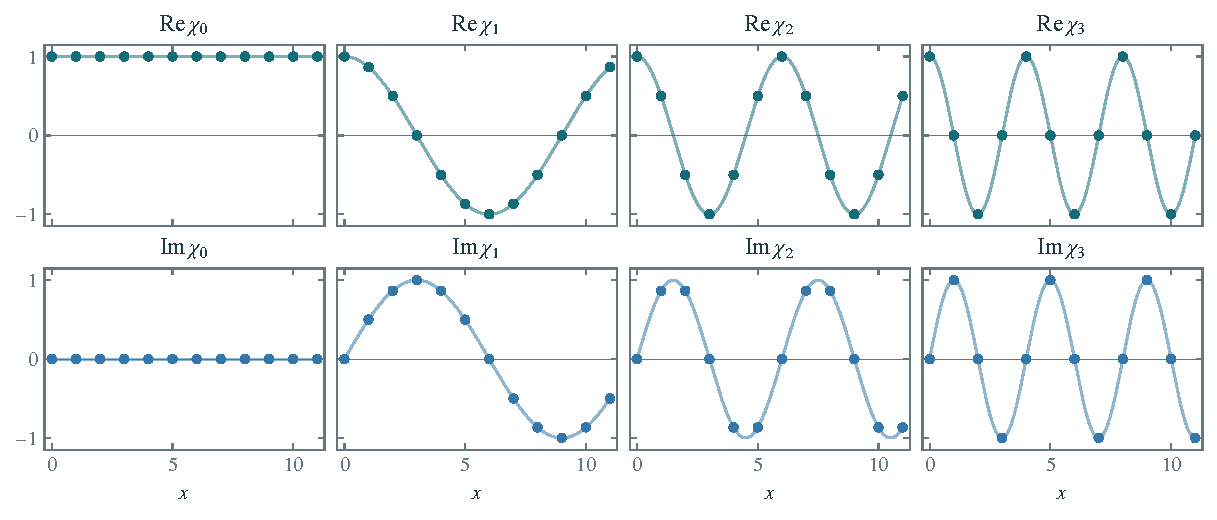
\includegraphics[width=\linewidth]{figures/chapter-finite-groups/cyclic-characters/figure.pdf}
\caption{Real and imaginary parts of the first four characters of $\ZZ/12\ZZ$.}
\label{fig-cyclic-characters}
\end{figure}

\begin{rem}
An abstract cyclic group has no preferred generator. Choosing a generator and
a primitive root of unity determines the isomorphism with its dual. This
choice dependence is analogous to the choice of a basis when identifying a
vector space with its dual.
\end{rem}

\begin{rem}
\label{rmk-zpz-isomorphism}
Every cyclic group of order $n$ is isomorphic to $\ZZ/n\ZZ$. For this concrete
group, the pairing $(j,k)\mapsto e^{2\pi\imath jk/n}$ gives the familiar
identification
\[
 \widehat{\ZZ/n\ZZ}\simeq\ZZ/n\ZZ.
\]
The structure theorem will extend the existence of such an isomorphism to
all finite abelian groups.
\end{rem}

\begin{prop}
\label{prop-base-ortho-cyclic-case}\label{notation-14}
\index{Orthogonality}\index{Kronecker symbol}
For a cyclic group $G$, the characters form an orthonormal basis of $\CC[G]$:
$\dotp{\chi_p}{\chi_q}=\delta_p^q$, where $\delta_p^q$ is $1$ if $p=q$ and $0$
otherwise.
\end{prop}
\begin{proof}
Using the preceding notation,
\begin{equation}
\label{eq-orthogonalite-cyclic-case}
 \dotp{\chi_p}{\chi_q}
 =\frac1n\sum_{k=0}^{n-1}\omega^{(p-q)k}=\delta_p^q.
\end{equation}
For $p\neq q$, the sum is a geometric series with ratio
$\omega^{p-q}\neq1$ and vanishes. For $p=q$, every summand is $1$.
There are $n$ orthonormal characters in an $n$-dimensional space, so they form
a basis.
\end{proof}

\section{Dual of an abelian group}
\label{sect1-dual-abelien-group}
We now prove that the characters of any finite abelian group form an
orthonormal basis. The key algebraic step is extension of a character from a
subgroup to the whole group.

\subsection{Character extension}
\label{sec2-approach-algebraic-dual-abelien}
\begin{lem}[Character extension]
\label{lem-prolongation-caractere}
\index{Character!extension}
Let $H$ be a subgroup of a finite abelian group $G$. Every character of $H$
extends to a character of $G$.
\end{lem}
\begin{proof}
\label{notation-15}
We induct on the index $[G:H]$. There is nothing to prove when $H=G$.
Otherwise, choose $x\in G\setminus H$ and let $K=\langle H,x\rangle$.
Let $n$ be the smallest positive integer such that $x^n\in H$; thus
$n=[K:H]\geq2$.

Every element of $K$ has a unique expression $yx^k$, with $y\in H$ and
$0\leq k<n$. Existence follows by reducing the exponent modulo $n$.
For uniqueness, $yx^k=y'x^{k'}$ implies $x^{k-k'}\in H$; the minimality
of $n$ and $|k-k'|<n$ force $k=k'$ and then $y=y'$.

Given $\chi\in\wh H$, choose a complex number $\zeta$ satisfying
$\zeta^n=\chi(x^n)$. Such a root exists and has modulus one. Define
\begin{equation}
\label{eq-formula-extension-character}
 \wt\chi(yx^k)=\chi(y)\zeta^k,\qquad y\in H,\quad 0\leq k<n.
\end{equation}
This is well defined by uniqueness and agrees with $\chi$ on $H$.
To check multiplicativity, write $k+k'=qn+r$, with $q\in\{0,1\}$ and
$0\leq r<n$. Since $G$ is abelian,
\begin{align*}
 \wt\chi\big((yx^k)(y'x^{k'})\big)
 &=\chi(yy'x^{qn})\zeta^r\\
 &=\chi(y)\chi(y')\chi(x^n)^q\zeta^r\\
 &=\chi(y)\chi(y')\zeta^{k+k'}
 =\wt\chi(yx^k)\wt\chi(y'x^{k'}).
\end{align*}
Thus $\wt\chi$ is a character of $K$. Finally,
$[G:K]=[G:H]/n<[G:H]$, so the induction hypothesis extends it to $G$.
\end{proof}
The root must satisfy $\zeta^n=\chi(x^n)$; it need not be an $n$th root of
\emph{unity}. For example, if $G=\langle x\rangle$ has order $4$,
$H=\{1,x^2\}$, and $\chi(x^2)=-1$, then $\zeta$ must be $\imath$ or
$-\imath$. In general, an extension is not unique.

\begin{lem}
\label{lem-suite-exact}\index{Sequence!exact}
For a subgroup $H$ of a finite abelian group $G$, restriction
$\rho:\wh G\to\wh H$ and pullback $j:\widehat{G/H}\to\wh G$,
$j(\eta)(x)=\eta(xH)$, give an exact sequence
\[
 \{1\}\longrightarrow\widehat{G/H}
 \overset{j}{\longrightarrow}\wh G
 \overset{\rho}{\longrightarrow}\wh H\longrightarrow\{1\}.
\]
\end{lem}
\begin{proof}
The quotient map $G\to G/H$ is surjective, so its pullback $j$ is injective.
Character extension makes $\rho$ surjective. A character lies in
$\Ker\rho$ precisely when it is trivial on $H$, in which case it factors
uniquely through $G/H$. Hence $\Ker\rho=\Im j$.
\end{proof}

\begin{cor}
\label{cor-order-dual-equal-order-group}
A finite abelian group and its dual have the same order.
\end{cor}
\begin{proof}
Induct on $|G|$. The result holds for cyclic groups, including the trivial
group. Otherwise choose a nontrivial proper cyclic subgroup $H$. Exactness
and the induction hypothesis give
\[
 |\wh G|=|\widehat{G/H}|\,|\wh H|=|G/H|\,|H|=|G|.
\]
\end{proof}

\subsection{Isomorphism with the dual}
\label{sect2-thm-isomorphism}
Equality of orders suffices for the orthogonality argument below. A stronger
statement follows from the structure theorem for finite abelian groups;
see Artin~\cite{artin} for a proof.

\begin{thm}[Structure theorem for finite abelian groups]
\label{thm-structure-abelian-groups}
There is a unique sequence of integers $2\leq n_1\mid n_2\mid\cdots\mid n_r$
such that
\[
 G\simeq\ZZ/n_1\ZZ\times\cdots\times\ZZ/n_r\ZZ.
\]
For the trivial group, the sequence is empty. The integers are unique;
the isomorphism generally is not.
\end{thm}

\begin{cor}[Isomorphism theorem]
\label{cor-thm-isomorphism}
Every finite abelian group $G$ is isomorphic to $\wh G$.
\end{cor}
\begin{proof}
There is a canonical isomorphism
$\widehat{G\times H}\simeq\wh G\times\wh H$: restrict a character to each
factor. Its inverse sends $(\chi,\eta)$ to
$(g,h)\mapsto\chi(g)\eta(h)$. Apply this to the cyclic factors in the
structure theorem and use Proposition~\ref{prop-cyclic-case}.
\end{proof}

\begin{rem}
The proof requires a choice of cyclic decomposition and generators. It gives
an isomorphism $G\simeq\wh G$, but no preferred identification for an arbitrary
finite abelian group. The situation changes when we pass to the bidual.
\end{rem}

\subsection{The bidual}
\label{sect2-bidual}
\begin{defn}[Bidual]
\label{notation-16}\index{Bidual}
The \emph{bidual} of a finite abelian group $G$ is
$\whwh G=\widehat{\wh G}$.
\end{defn}

\begin{prop}[Canonical isomorphism]
Evaluation gives a canonical isomorphism
\begin{equation}
\label{eq-inj-canonical}
 \Phi:G\longrightarrow\whwh G,\qquad
 \Phi(g)(\chi)=\chi(g).
\end{equation}
\end{prop}
\begin{proof}
For each $g$, evaluation is a character of $\wh G$, and
$\Phi(gh)=\Phi(g)\Phi(h)$. To prove injectivity, let $g\neq1$ have order $m$.
On $\langle g\rangle$, the character sending $g$ to $e^{2\pi\imath/m}$
is nontrivial at $g$. Extend it to $G$ using
Lemma~\ref{lem-prolongation-caractere}. Therefore $\Phi(g)\neq1$.
Since $|G|=|\whwh G|$, injectivity implies surjectivity.
\end{proof}

\begin{rem}
This is the analogue of the canonical map from a finite-dimensional vector
space to its double dual. For infinite groups, the choice of characters and
topology matters. With continuous unit-modulus characters, Pontryagin duality
extends the bidual theorem to locally compact abelian groups. For example,
the dual of $\RR/(2\pi\ZZ)$ is $\ZZ$, and the dual of $\ZZ$ is again the
circle. The fact that a group differs from its \emph{dual} does not prevent
its canonical identification with its \emph{bidual}.
\end{rem}

\subsection{Orthogonality relations}
\label{sect2-dual-grpe-abelien-rel-orthogonalite}
\begin{lem}
\label{lem-orth-character-abelien}
For a character $\chi$ of a finite abelian group $G$,
\begin{equation}
\label{eq-sum-caracteres-grpe-abelien}
 \sum_{g\in G}\chi(g)=
 \begin{cases}|G|&\chi=1,\\0&\chi\neq1.\end{cases}
\end{equation}
\end{lem}
\begin{proof}
The trivial character gives the first case. Otherwise choose $t$ with
$\chi(t)\neq1$. Translation permutes the summation indices, so
\[
 \chi(t)\sum_{g\in G}\chi(g)
 =\sum_{g\in G}\chi(tg)=\sum_{g\in G}\chi(g).
\]
Subtracting and dividing by $\chi(t)-1$ gives the second case.
\end{proof}

\begin{prop}[Orthogonality of characters]
\label{prop-orthogonalite-car-grpe-abelien}
For $\chi_1,\chi_2\in\wh G$,
\[
 \dotp{\chi_1}{\chi_2}=\begin{cases}1&\chi_1=\chi_2,\\0&\chi_1\neq\chi_2.\end{cases}
\]
\end{prop}
\begin{proof}
Apply the preceding lemma to the character $\chi_1\ol{\chi_2}$.
It is trivial exactly when $\chi_1=\chi_2$.
\end{proof}

\begin{cor}
The characters of a finite abelian group $G$ form an orthonormal basis of
$\CC[G]$.
\end{cor}
\begin{proof}
They are orthonormal, and their number is $|G|=\dim_{\CC}\CC[G]$.
\end{proof}

\begin{prop}[Dual orthogonality]
\label{prop-relations-orthogonalite-duale-grpe-abelien}
For $g,h\in G$,
\[
 \sum_{\chi\in\wh G}\chi(g)\ol{\chi(h)}=|G|\delta_g^h.
\]
\end{prop}
\begin{proof}
Apply character orthogonality to $\wh G$ and the evaluation characters
$\Phi(g),\Phi(h)$. This gives
\begin{equation}
\label{eq-rel-orth-col-temp}
 \sum_{\chi\in\wh G}\Phi(g)(\chi)\ol{\Phi(h)(\chi)}
 =|\wh G|\delta_{\Phi(g)}^{\Phi(h)}=|G|\delta_g^h.
\end{equation}
\end{proof}

\begin{rem}
Enumerate $G=\{g_1,\ldots,g_n\}$ and
$\wh G=\{\chi_1,\ldots,\chi_n\}$. For the character table
$M_{ij}=\chi_i(g_j)$, the two orthogonality relations read
$MM^*=M^*M=nI$. Thus $M/\sqrt n$ is unitary. The two identities express
orthogonality of the rows and columns, respectively.
\end{rem}

\section{Dual of a noncommutative group}
\label{sect1-dual-non-commutative-group}
For noncommutative groups, linear characters no longer suffice to represent
all functions. The symmetric group gives a concrete example; its
abelianization explains the general obstruction.

\subsection{The symmetric group}
\label{sect2-exmp-dual-sn}\label{notation-17}
\index{Symmetric group}
\begin{defn}[Sign of a permutation]
\index{Sign!of a permutation}
Write $\sigma\in\mathfrak S_n$ as a product of disjoint cycles, including
cycles of length one. If there are $k$ cycles, its \emph{sign} is
\[
 \epsilon(\sigma)=(-1)^{n-k}.
\]
\end{defn}
Uniqueness of disjoint cycle decomposition makes this definition unambiguous;
see Lang~\cite{lang}.

\begin{lem}
For a transposition $\tau$, one has $\epsilon(\sigma\tau)=-\epsilon(\sigma)$.
\end{lem}
\begin{proof}
Write $\tau=(a,b)$. If $a$ and $b$ belong to the same cycle of $\sigma$,
right multiplication by $\tau$ splits that cycle into two. Otherwise it joins
their two cycles. In either case the number of cycles changes by one.
\end{proof}

\begin{prop}
If $\sigma$ is a product of $p$ transpositions, then
$\epsilon(\sigma)=(-1)^p$. Moreover, $\epsilon$ is a homomorphism
$\mathfrak S_n\to\{1,-1\}$.
\end{prop}
\begin{proof}
Starting from the identity, apply the preceding lemma $p$ times.
Concatenating decompositions of two permutations then proves multiplicativity.
\end{proof}
Although a transposition decomposition is not unique, its parity is therefore
well defined. An alternative definition is the determinant of the permutation
matrix.

\begin{prop}
For $n\geq2$, the only nontrivial linear character of $\mathfrak S_n$ is its
sign $\epsilon$.
\end{prop}
\begin{proof}
Transpositions generate $\mathfrak S_n$ and are all conjugate, so a character
has a common value $a$ on them. Since a transposition squares to the identity,
$a^2=1$. If $a=1$, the character is trivial. If $a=-1$, its value on a product
of $p$ transpositions is $(-1)^p$, so it equals $\epsilon$.
\end{proof}
Thus $\widehat{\mathfrak S_n}\simeq\ZZ/2\ZZ$ for $n\geq2$. For $n=1$, both
$\mathfrak S_1$ and its dual are trivial.

\subsection{The derived subgroup}
\begin{defn}[Derived subgroup]
\label{notation-18}\label{notation-19}
\index{Commutator}\index{Group!derived subgroup}
The \emph{commutator} of $x,y\in G$ is $[x,y]=xyx^{-1}y^{-1}$.
The subgroup generated by all commutators,
\[
 D(G)=\langle[x,y]:x,y\in G\rangle,
\]
is the \emph{derived subgroup} (or commutator subgroup).
\end{defn}

\begin{prop}[Properties of the derived subgroup]
\label{prop-pte-grpe-derive}
The subgroup $D(G)$ is normal, $G/D(G)$ is abelian, and $D(G)=\{1\}$ if and
only if $G$ is abelian.
\end{prop}
\begin{proof}
Every automorphism $\varphi$ satisfies
$\varphi([x,y])=[\varphi(x),\varphi(y)]$ and therefore preserves $D(G)$.
In particular, inner automorphisms preserve it, proving normality.
In the quotient, $\ol x\,\ol y\,\ol x^{-1}\ol y^{-1}=1$, so all elements
commute. Finally, all commutators are trivial exactly when $G$ is abelian.
\end{proof}

\begin{prop}
\label{prop-descr-dual-grpe-derive}
For a finite group $G$, there is a canonical isomorphism
$\wh G\simeq\widehat{G/D(G)}$. Consequently,
$\wh G\simeq G/D(G)$, with the second isomorphism generally depending on choices.
\end{prop}
\begin{proof}
The target $\CC^*$ is abelian, so every character is trivial on commutators
and hence on $D(G)$. It therefore factors uniquely through the quotient:
\[
 \ol\chi(xD(G))=\chi(x).
\]
Conversely, pullback along $G\to G/D(G)$ gives a character of $G$.
These constructions are inverse homomorphisms. Since $G/D(G)$ is finite
abelian, Corollary~\ref{cor-thm-isomorphism} gives the final assertion.
\end{proof}

\begin{rem}
The factorization is expressed by the commutative diagram
\[
 \begin{CD}
 G @>{\chi}>> \CC^*\\
 @V{\pi}VV @|\\
 G/D(G) @>{\ol\chi}>> \CC^*.
 \end{CD}
\]
In particular, $|\wh G|=|G|/|D(G)|$. When $G$ is nonabelian this is strictly
less than $|G|$, so linear characters cannot span $\CC[G]$.
\end{rem}

\label{notation-20}\index{Alternating group}
The alternating group $\mathfrak A_n=\Ker\epsilon$ is the normal subgroup of
even permutations.
\begin{lem}
For $n\geq3$, the group $\mathfrak A_n$ is generated by $3$-cycles.
\end{lem}
\begin{proof}
The transpositions $(1,i)$ generate $\mathfrak S_n$, since
$(i,j)=(1,i)(1,j)(1,i)$ for distinct $i,j\neq1$. An even permutation is a
product of an even number of these transpositions. Group them into pairs.
A pair of equal transpositions is the identity; a pair of distinct ones is a
$3$-cycle.
\end{proof}

\begin{prop}[The symmetric group]
For $n\geq3$, $D(\mathfrak S_n)=\mathfrak A_n$ and
$\widehat{\mathfrak S_n}\simeq\mathfrak S_n/\mathfrak A_n\simeq\ZZ/2\ZZ$.
\end{prop}
\begin{proof}
Since $\epsilon$ is a character, $D(\mathfrak S_n)\subset\mathfrak A_n$.
For a $3$-cycle $\sigma$, choose $\tau$ with
$\tau\sigma\tau^{-1}=\sigma^2$; for instance, exchange two entries of the
cycle. Then $[\tau,\sigma]=\sigma$. The preceding lemma gives the reverse
inclusion. The quotient is isomorphic to $\{1,-1\}$ by the sign map.
\end{proof}

\begin{rem}
To recover Fourier analysis on a noncommutative group, we replace scalar-valued
homomorphisms by matrix-valued representations. Linear characters correspond
to representations of dimension one. Higher-dimensional representations
supply the missing components; this is the subject of
Chapter~\ref{chap-linear-representations-finite-groups}.
\end{rem}

\section{The Fourier transform}
\label{sect1-transforme-fourier}
Throughout this section, $G$ is a finite abelian group. Its character basis
now gives a systematic decomposition of every function on $G$.

\subsection{Fourier coefficients and the Fourier transform}
\label{sect2-coef-fourier-transforme-fourier}
\begin{defn}[Fourier coefficients]
\label{notation-21}\index{Fourier coefficient}
For $f\in\CC[G]$ and $\chi\in\wh G$, define
\[
 c_f(\chi)=\dotp f\chi
 =\frac1{|G|}\sum_{x\in G}f(x)\ol{\chi(x)}.
\]
This defines a linear map $c:\CC[G]\to\CC[\wh G]$, $f\mapsto c_f$.
\end{defn}

\begin{defn}[Fourier transform]
\label{notation-22}
The Fourier transform is the linear map
\begin{equation}
\label{eq-transf-fourier-grpe-abelien}
 \Ff:\CC[G]\longrightarrow\CC[\wh G],\qquad f\longmapsto\wh f,
 \qquad \wh f(\chi)=\sum_{x\in G}f(x)\chi(x).
\end{equation}
Thus $\wh f(\chi)=|G|c_f(\ol\chi)$.
\end{defn}
This convention makes evaluation of $\wh f$ an algebra homomorphism for
convolution. The numerical DFT in Chapter~\ref{chap-tfd} uses a negative
exponential: it is the same transform evaluated at the inverse cyclic
characters $\chi_k^{-1}(x)=e^{-2\pi\imath kx/n}$. Keeping track of this
indexing choice avoids sign ambiguities.

Figure~\ref{fig-decomposition-fourier} shows a bell-shaped function on
$\ZZ/17\ZZ$ and its transform, with centered indices $-8,\ldots,8$.
The coefficient of the trivial character is the sum of the function values.

\begin{figure}[tbp]
\centering
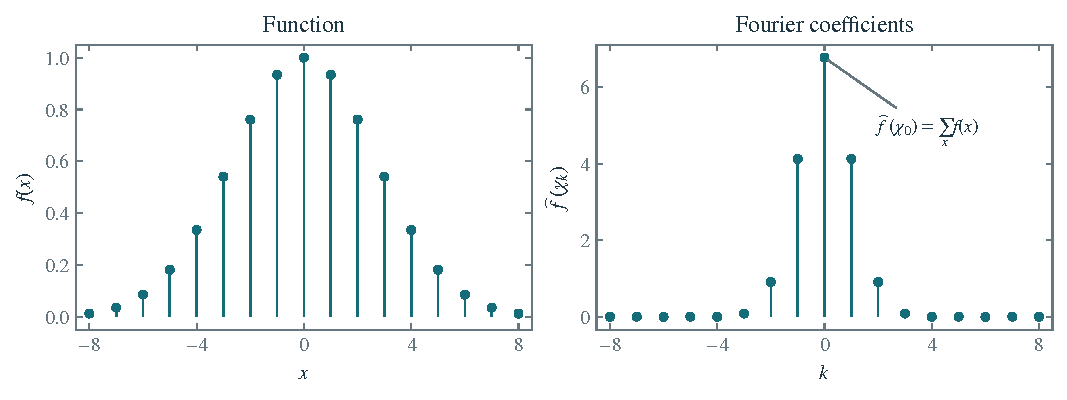
\includegraphics[width=\linewidth]{figures/chapter-finite-groups/fourier-decomposition/figure.pdf}
\caption{An even bell-shaped function on $\ZZ/17\ZZ$ and its real Fourier coefficients, with centered indices.}
\label{fig-decomposition-fourier}
\end{figure}

\begin{prop}[Inversion formula]
\label{prop-decomposition-serie-fourier}\index{Fourier!inversion}
For every $f\in\CC[G]$,
\begin{equation}
\label{eq-decomposition-serie-fourier-grpe-abelien}
 f=\sum_{\chi\in\wh G}c_f(\chi)\chi
 =\frac1{|G|}\sum_{\chi\in\wh G}\wh f(\chi)\chi^{-1}.
\end{equation}
\end{prop}
\begin{proof}
The first equality is expansion in the orthonormal character basis.
For the second, substitute $c_f(\chi)=\wh f(\chi^{-1})/|G|$ and reindex by
$\chi\mapsto\chi^{-1}$.
\end{proof}

\begin{prop}[Fourier isomorphism]
The maps $c$ and $\Ff$ are vector-space isomorphisms
$\CC[G]\to\CC[\wh G]$.
\end{prop}
\begin{proof}
Inversion gives injectivity. The domain and codomain both have dimension
$|G|$, so the maps are also surjective.
\end{proof}

\begin{prop}[Plancherel's formula]
\label{prop-formula-floorel}\index{Plancherel's formula}
For $f,g\in\CC[G]$,
\begin{align}
\label{eq-formula-floorel-grpe-abelien-1}
 \sum_{x\in G}f(x)\ol{g(x)}
 &=|G|\sum_{\chi\in\wh G}c_f(\chi)\ol{c_g(\chi)}\\
\label{eq-formula-floorel-grpe-abelien-2}
 &=\frac1{|G|}\sum_{\chi\in\wh G}\wh f(\chi)\ol{\wh g(\chi)}.
\end{align}
\end{prop}
\begin{proof}
Expand both functions in the orthonormal character basis. Orthogonality
eliminates all terms involving distinct characters and gives the first
identity. The relation between $c_f$ and $\wh f$ gives the second.
\end{proof}

\begin{rem}[Normalization]
With the normalized inner products on both $\CC[G]$ and $\CC[\wh G]$,
Plancherel's formula reads
\[
 \dotp fg=\frac1{|G|}\dotp{\wh f}{\wh g}.
\]
Thus $\Ff/\sqrt{|G|}$ is unitary. This is the finite analogue of conservation
of the $L^2$ inner product by a suitably normalized continuous Fourier
transform; see Section~\ref{sect1-link-trans-fourier-R}.
\end{rem}

\subsection{The group algebra}
\label{sect2-algebre-grpe-abelien}
\index{Algebra!group algebra}\index{Convolution}
The pointwise product
\begin{equation}
\label{eq-defn-prod-term-term-functions}
 (f_1\cdot f_2)(g)=f_1(g)f_2(g)
\end{equation}
turns $\CC[G]$ into an algebra, but does not use multiplication in $G$.
A second product does: set $\delta_g*\delta_h=\delta_{gh}$ and extend by
bilinearity. Expanding two functions in the Dirac basis gives the following
formula.

\begin{defn}[Convolution]
\label{notation-23}
For $f_1,f_2\in\CC[G]$, their convolution is
\begin{equation}
\label{eq-formula-prod-convol-grpe-abelien}
 (f_1*f_2)(g)=\sum_{hk=g}f_1(h)f_2(k)
 =\sum_{h\in G}f_1(h)f_2(h^{-1}g).
\end{equation}
\end{defn}

\begin{rem}
Convolution with a Dirac function translates a function:
$(f*\delta_g)(h)=f(hg^{-1})$.
For cyclic groups this is circular translation, studied in
Section~\ref{sect1-tfd-prod-convol}.
\end{rem}

\begin{prop}
Convolution is bilinear, associative, and commutative, with identity $\delta_1$.
It makes $\CC[G]$ a commutative unital algebra.
\end{prop}
\begin{proof}
Bilinearity is part of the construction. On basis elements,
\[
 (\delta_g*\delta_h)*\delta_k=\delta_{(gh)k}
 =\delta_{g(hk)}=\delta_g*(\delta_h*\delta_k).
\]
Bilinearity extends associativity to all functions. Commutativity follows
from $gh=hg$, and $\delta_1*\delta_g=\delta_g$ proves the identity property.
\end{proof}
Figure~\ref{fig-convolution-intro} illustrates self-convolution of a box signal
on $\ZZ/16\ZZ$. The values count overlaps of translated supports. This
viewpoint connects direct summation, FFT computation in Python, and
multiplication of polynomials modulo $X^{16}-1$.

\begin{figure}[tbp]
\centering
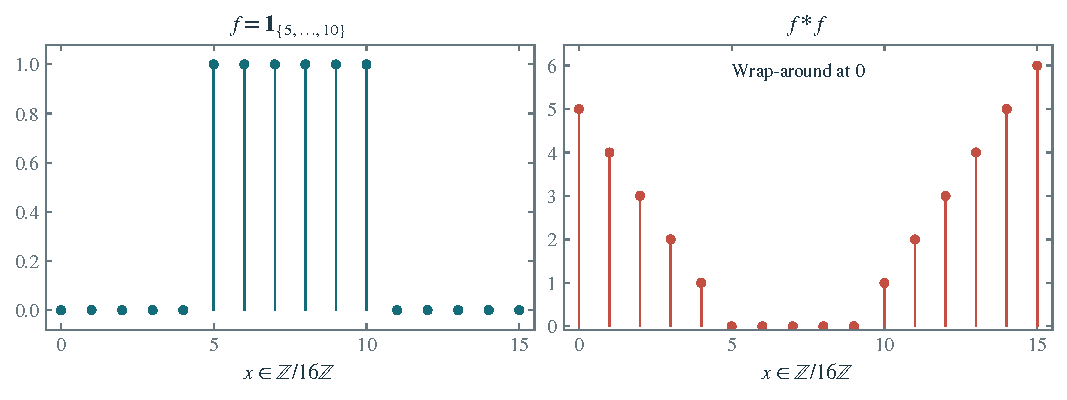
\includegraphics[width=\linewidth]{figures/chapter-finite-groups/circular-convolution/figure.pdf}
\caption{Circular self-convolution of $f=\mathbf{1}_{\{5,\ldots,10\}}$ on $\ZZ/16\ZZ$. The maximum occurs at $15$ modulo $16$; the remaining values wrap around at $0$.}
\label{fig-convolution-intro}
\end{figure}

\begin{prop}[Extension to the group algebra]
\label{prop-extension-morphism-grpe-algebra}
Every homomorphism $\rho:G\to\CC^*$ extends uniquely to a unital
$\CC$-algebra homomorphism $\wt\rho:\CC[G]\to\CC$.
\end{prop}
\begin{proof}
Linearity forces
$\wt\rho(f)=\sum_{g\in G}f(g)\rho(g)$.
Since $\rho(gh)=\rho(g)\rho(h)$, this extension preserves products of basis
elements and hence all convolution products. It maps $\delta_1$ to $1$.
\end{proof}
Conversely, a unital algebra homomorphism restricts to a group homomorphism on
the invertible elements $\delta_g$. The word \emph{unital} excludes the zero
homomorphism, which cannot take values in $\CC^*$.

\begin{rem}[Probabilistic interpretation]
\label{rmk-interpretation-proba}\index{Probability}
Let $X,Y$ be independent $G$-valued random variables, with probability mass
functions $P_X,P_Y$. Independence gives
\[
 \PP(XY=g)=\sum_{h\in G}\PP(X=h)\PP(Y=h^{-1}g)
 =(P_X*P_Y)(g).
\]
In additive notation this is $P_{X+Y}=P_X*P_Y$. Analogous formulas hold for
integer-valued variables and for real-valued variables with densities;
see Ouvrard~\cite{ouvrard-2}.
Exercises~\ref{exo-repartition-proba} and~\ref{exo-marche-aleatoire} develop
finite-group applications.
\end{rem}

\subsection{Convolution and the Fourier transform}
\label{sect2-convolution-transforme-fourier}
\begin{prop}[Fourier evaluation as an algebra homomorphism]
\label{prop-thm-convol-fourier-grpe-finite}
For each $\chi\in\wh G$, the map
$\Ff_\chi:f\mapsto\wh f(\chi)$ is the unique unital algebra homomorphism
extending $\chi$ to $\CC[G]$.
\end{prop}
\begin{proof}
The extension formula in Proposition~\ref{prop-extension-morphism-grpe-algebra}
is precisely $\wh f(\chi)=\sum_g f(g)\chi(g)$.
\end{proof}

\begin{thm}[Convolution theorem]
\label{thm-convolution-trans-fourier-grpe-abelien}
For $f,g\in\CC[G]$,
\begin{equation}
\label{eq-formula-convolution-functions-abelien-grpe}
 \widehat{f*g}=\wh f\cdot\wh g,
 \qquad c_{f*g}=|G|c_f\cdot c_g.
\end{equation}
The Fourier transform is an algebra isomorphism from $(\CC[G],*)$ to
$(\CC[\wh G],\cdot)$.
\end{thm}
\begin{proof}
The first identity holds at every $\chi$ by the preceding proposition.
The second follows from $\wh f(\chi)=|G|c_f(\ol\chi)$.
Inversion supplies the isomorphism assertion.
\end{proof}
Convolution has become pointwise multiplication. This simple structural fact
will underlie fast filtering, polynomial multiplication, spectral solutions
of differential equations, and the decoding of error-correcting codes.

\section{Exercises}
\label{sect1-chap1-exercises}

\begin{exo}[Circulant determinant]
\label{exo-determinant-circulating}\index{Determinant!circulant}
Let $G$ be cyclic and $f\in\CC[G]$. Consider the convolution operator
$\Phi^f(u)=f*u$ on $\CC[G]$.
\begin{enumerate}
\item Show that every character is an eigenvector of $\Phi^f$. Find the
corresponding eigenvalue, keeping track of the Fourier sign convention.
\item Express the matrix $A$ of $\Phi^f$ in the Dirac basis and deduce a
formula for $\det A$.
\item With $\omega=e^{2\pi\imath/n}$, show that
\[
 \det\begin{pmatrix}
 a_0&a_1&\cdots&a_{n-1}\\
 a_{n-1}&a_0&\cdots&a_{n-2}\\
 \vdots&\vdots&\ddots&\vdots\\
 a_1&a_2&\cdots&a_0
 \end{pmatrix}
 =\prod_{i=0}^{n-1}\left(\sum_{j=0}^{n-1}a_j\omega^{ij}\right).
\]
\item After reading Chapter~\ref{chap-tfd}, implement this determinant using
an FFT. Discuss the numerical limitations of multiplying many eigenvalues.
\end{enumerate}
\end{exo}

\begin{exo}[Linear characters of $SO(3)$]
\label{exo-dual-so3}\index{Rotation}
Let $SO(3)$ be the group of real orthogonal $3\times3$ matrices of determinant
one. Show that every homomorphism $SO(3)\to\CC^*$ is trivial.
\begin{enumerate}
\item Prove that rotations with the same angle in $[0,\pi]$ are conjugate.
\item Deduce that a character $\chi$ depends only on the rotation angle.
\item Let $r_\alpha$ and $s_\alpha$ be rotations through $\alpha$ about the
first and second coordinate axes. Show that $r_\alpha s_\alpha^{-1}$ is a
rotation through an angle $\beta$ satisfying
$\cos\beta=((1+\cos\alpha)^2-2)/2$.
As $\alpha$ varies over $[0,\pi]$, show that $\beta$ covers $[0,\pi]$.
\item Deduce that $\chi=1$. No continuity assumption on $\chi$ is needed.
\end{enumerate}
\end{exo}

\begin{exo}[Counting solutions]
\label{exo-enombrement-solutions}\index{Counting}
Let $G$ be finite abelian and $\varphi:G^n\to G$ any map. For $h\in G$, let
$N(h)$ count the tuples satisfying $\varphi(g_1,\ldots,g_n)=h$. Prove that
\[
 N(h)=\frac1{|G|}\sum_{g_1,\ldots,g_n\in G}
       \sum_{\chi\in\wh G}\chi\big(\varphi(g_1,\ldots,g_n)\big)\ol{\chi(h)}.
\]
\end{exo}

\begin{exo}[Indicator functions]
\label{exo-indicator-functions}\index{Function!indicator}
Let $G$ be finite abelian with $|G|\geq2$, and let $f_A$ be the indicator of
$A\subset G$. Write $\chi_0$ for the trivial character.
\begin{enumerate}
\item Show that $\norm{f_A}_2=\sqrt{|A|/|G|}$ and $\wh f_A(\chi_0)=|A|$.
\item Define
\begin{equation}
\label{eq-defn-phi-ensemble}
 \Phi(A)=\max_{\chi\neq\chi_0}|\wh f_A(\chi)|.
\end{equation}
If $|A|\leq|G|/2$, prove that
\begin{equation}
\label{eq-ineq-regularity-function-indic}
 \sqrt{|A|/2}\leq\Phi(A)\leq|A|.
\end{equation}
\item Show that $\Phi(A)=\Phi(G\setminus A)$ and obtain corresponding bounds
when $|A|>|G|/2$.
\item Prove that $\Phi(\alpha(A))=\Phi(A)$ for every automorphism $\alpha$.
Using additive notation, also prove $\Phi(A+a)=\Phi(A)$ for every $a\in G$.
\end{enumerate}
Small nontrivial Fourier coefficients indicate that $A$ has little correlation
with any nonconstant character. This form of uniform distribution will be
useful in counting problems and coding theory.
\end{exo}

\begin{exo}[Equations on a finite abelian group]
\label{exo-eqn-grpe-abelien-finite}
Use the notation of Exercise~\ref{exo-indicator-functions}. The argument is
adapted from Babai~\cite{babai-fourier-equations}.
\begin{enumerate}
\item For subsets $A_1,\ldots,A_k\subset G$, consider
\begin{equation}
\label{eq-exo-nbr-solution-eqn-grpe-finite}
 x_1+\cdots+x_k=a,\qquad x_i\in A_i.
\end{equation}
Reduce to $a=0$ by translating one set. For $a=0$, show that the number of
solutions is
\[
 N=\frac{|A_1|\cdots|A_k|}{|G|}+R,\qquad
 R=\frac1{|G|}\sum_{\chi\neq\chi_0}\prod_{i=1}^k\wh f_{A_i}(\chi).
\]
\item For $k=3$, use Cauchy--Schwarz and Plancherel to prove
\[
 |R|\leq\frac{\Phi(A_3)}{|G|}
 \sum_{\chi\in\wh G}|\wh f_{A_1}(\chi)|\,|\wh f_{A_2}(\chi)|
 \leq\Phi(A_3)\sqrt{|A_1|\,|A_2|}.
\]
Explain why the same bound holds for general $a$.
\item For nonempty $A_1,A_2,A_3$, deduce that a solution exists for every
$a\in G$ if
\[
 \frac{\Phi(A_3)}{|A_3|}<\frac{\sqrt{|A_1|\,|A_2|}}{|G|}.
\]
\end{enumerate}
Exercise~\ref{exo-thm-fermat-finite-body} applies this criterion over a finite
field to an analogue of Fermat's equation.
\end{exo}

\begin{exo}[The Heisenberg group]
\label{exo-groupe-heisenberg}\index{Heisenberg group}
Let $G$ be finite abelian and $\Uu=\{z\in\CC:|z|=1\}$. On
$\Hh(G)=\Uu\times G\times\wh G$, define
\[
 (\lambda,x,\chi)(\mu,y,\tau)
 =(\lambda\mu\tau(x),xy,\chi\tau).
\]
\begin{enumerate}
\item Verify the group axioms and find the identity and inverses.
\item Show that
$((\lambda,x,\chi)\cdot f)(z)=\lambda\chi(z)f(xz)$
defines an action on $\CC[G]$.
\item Define scalar multiplication $D_\lambda f=\lambda f$, translation
$T_xf(z)=f(xz)$, and modulation $M_\chi f(z)=\chi(z)f(z)$.
Express the action using these operators and determine their Fourier
transforms. Compare with the corresponding operations on $\RR$.
\item Identify $G$ with its bidual. Write the product on
$\Hh(\wh G)=\Uu\times\wh G\times G$ and its action on $\CC[\wh G]$.
\item Prove that
\[
 \alpha(\lambda,x,\chi)=(\lambda\chi(x)^{-1},\chi,x^{-1})
\]
is an isomorphism $\Hh(G)\to\Hh(\wh G)$ and that
\[
 \Ff\big((\lambda,x,\chi)\cdot f\big)
 =\alpha(\lambda,x,\chi)\cdot\Ff(f).
\]
\item Let $\Phi:\CC[G]\to\CC[G]$ be \emph{complex-linear} and commute with
the action of $\Hh(G)$. Prove that $\Phi=rI$ for some $r\in\CC$.
One may use the Dirac basis or Schur's lemma (Lemma~\ref{lemma-schur}).
Deduce that a complex-linear map $\Psi:\CC[G]\to\CC[\wh G]$ satisfying
$\Psi(h\cdot f)=\alpha(h)\cdot\Psi(f)$ is a scalar multiple of $\Ff$.
When is this map invertible?
\end{enumerate}
\end{exo}

\begin{exo}[Fourier analysis and orthogonal translates]
\label{exo-series-fourier-orthogonalisation}
Let $f\in L^2(\RR)$ and $\tau_rf=f(\cdot-r)$. Use the convention
\[
 \wh f(\omega)=\int_{\RR}f(x)e^{-\imath\omega x}\,\d x
\]
for $f\in L^1\cap L^2$, extended to $L^2$ by density.
\begin{enumerate}
\item Prove that $(\tau_nf)_{n\in\ZZ}$ is orthonormal if and only if
\[
 \sum_{k\in\ZZ}|\wh f(\omega+2\pi k)|^2=1
 \quad\text{for almost every }\omega.
\]
\item\label{notation-24}
Suppose $S(\omega)=\sum_k|\wh f(\omega+2\pi k)|^2\geq A>0$ almost
 everywhere. Define $\varphi$ by
\[
 \wh\varphi(\omega)=\frac{\wh f(\omega)}{\sqrt{S(\omega)}}.
\]
Show that $\varphi\in L^2(\RR)$ and that its integer translates are orthonormal.
\end{enumerate}
The next exercise gives a finite-group counterpart.
\end{exo}

\begin{exo}[Orthogonalization on an abelian group]
\label{exo-orthogonalization-abelian-group}
Let $V$ be a finite-dimensional complex inner-product space, with inner
product linear in the first argument, and let $G$ be a finite abelian group
of unitary operators on $V$. For $b\in V$, call the \emph{indexed family}
$(Ab)_{A\in G}$ orthonormal when $\dotp{Ab}{Bb}=\delta_A^B$.
The indexing matters: repeated orbit vectors do not count as distinct
orthonormal vectors. See Bernardini and Kovacevic~\cite{bernardini-orthogonalisation-1}.
\begin{enumerate}
\item Set $\psi_b(A)=\dotp{Ab}{b}$ and
\[
 \Uu_\chi=\frac1{|G|}\sum_{A\in G}\chi(A)A.
\]
Show that $(Ab)_{A\in G}$ is orthonormal if and only if
$\wh\psi_b\equiv1$, equivalently
$|G|\dotp{\Uu_\chi b}{b}=1$ for every $\chi$.
\item Prove that the $\Uu_\chi$ are self-adjoint orthogonal projectors,
$\Uu_{\chi_1}\Uu_{\chi_2}=0$ for $\chi_1\neq\chi_2$, and
$\sum_\chi\Uu_\chi=I$. Deduce
$\wh\psi_b(\chi)=|G|\norm{\Uu_\chi b}^2\geq0$.
\item If $\wh\psi_b$ never vanishes, show that
\[
 \wt b=\sum_{\chi\in\wh G}
       \frac{\Uu_\chi b}{\sqrt{\wh\psi_b(\chi)}}
\]
has an orthonormal indexed orbit. Use the positive square roots.
\item Compare this construction with
Exercise~\ref{exo-series-fourier-orthogonalisation}. Explain why an orthonormal
orbit requires $|G|\leq\dim V$.
\end{enumerate}
\end{exo}

\begin{exo}[Distance from the uniform distribution]
\label{exo-repartition-proba}\index{Probability}
Let $P:G\to[0,1]$ be a probability mass function on a finite abelian group,
and let $U(g)=1/|G|$. Write $\chi_0$ for the trivial character.
\begin{enumerate}
\item Compute $\wh P(\chi_0)$ and $\wh U(\chi)$. Express
$\norm{P-U}_2^2$ using the nontrivial Fourier coefficients of $P$.
\item Prove that, for every $g\in G$,
\[
 \left|P(g)-\frac1{|G|}\right|^2
 \leq\frac1{|G|}\sum_{\chi\neq\chi_0}|\wh P(\chi)|^2.
\]
\end{enumerate}
The nontrivial coefficients quantify the departure from uniformity.
\end{exo}

\begin{exo}[Random walks]
\label{exo-marche-aleatoire}\index{Random walk}\index{Markov chain}
Consider a time-homogeneous random walk $(X_k)$ on $\ZZ/n\ZZ$, with $n\geq3$.
Write $p_{i,j}=\PP(X_{k+1}=j\mid X_k=i)$, and let $p^{(k)}$ be the column
vector with entries $p^{(k)}_i=\PP(X_k=i)$.
\begin{enumerate}
\item Define $P_{j,i}=p_{i,j}$, so each \emph{column} of $P$ sums to one.
Prove $p^{(k+1)}=Pp^{(k)}$ and $p^{(k)}=P^kp^{(0)}$.
In the remaining questions take $p^{(0)}=\delta_0$.
\item Let $0<p<1$, with $p_{i,i-1}=p$, $p_{i,i+1}=1-p$, and all other
transition probabilities zero. Show $Px=v*x$, where
$v(1)=1-p$, $v(-1)=p$, and $v$ vanishes elsewhere.
Recover the formula by adding an independent random increment.
\item Express $\wh p^{(k)}$ in terms of $\wh v$ and $\wh p^{(0)}$.
Show that $p^{(k)}$ tends to the uniform distribution if $n$ is odd.
Explain the parity obstruction when $n$ is even.
\item Generalize to $p_{i,j}=v(j-i)$ for a probability mass function $v$.
Give a necessary and sufficient condition for convergence to uniformity
from every initial distribution in terms of $|\wh v(\chi)|$ for nontrivial
characters. Interpret the role of characters that are constant on the support
of $v$.
\end{enumerate}
Figure~\ref{fig-marche-aleatoire} compares two increment distributions.
The magnitude of the largest nontrivial Fourier coefficient controls the
asymptotic rate of convergence when that magnitude is less than one.

\begin{figure}[tbp]
\centering
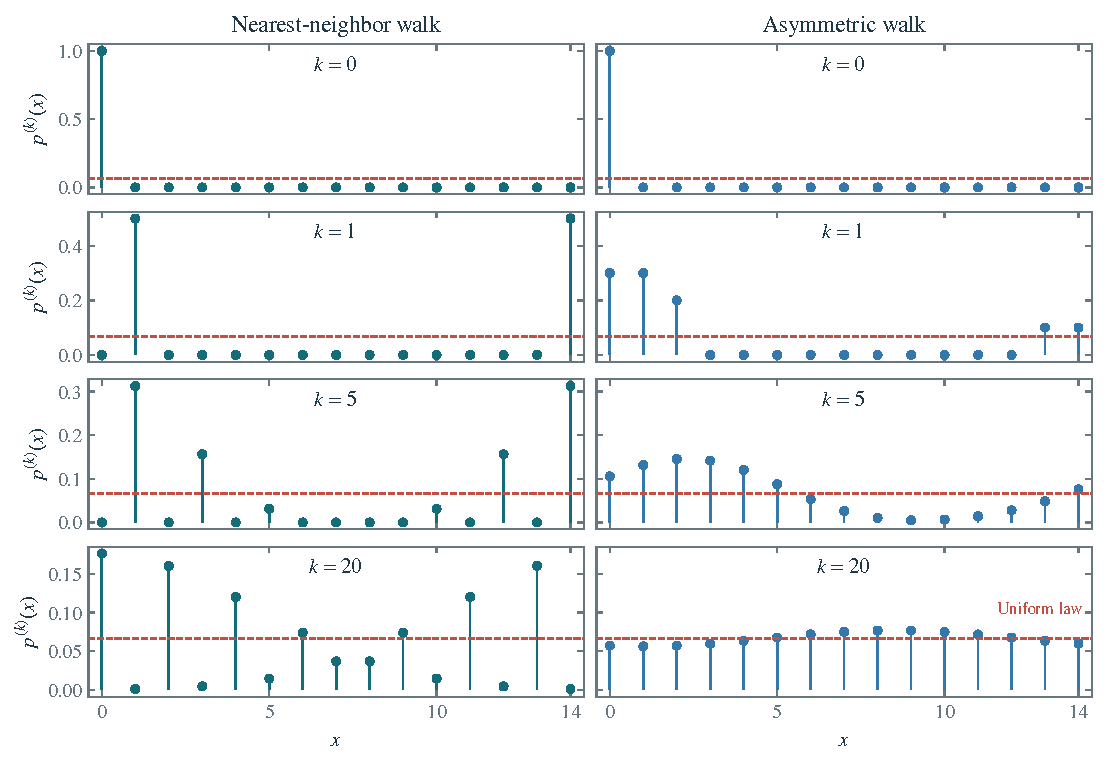
\includegraphics[width=\linewidth]{figures/chapter-finite-groups/random-walks/figure.pdf}
\caption{Random walks on $\ZZ/15\ZZ$ with increment laws $(0,1/2,0,\ldots,0,1/2)$ and $(0.3,0.3,0.2,0,\ldots,0,0.1,0.1)$. Dashed lines show the uniform distribution.}
\label{fig-marche-aleatoire}
\end{figure}
\end{exo}

\begin{exo}[The discrete uncertainty principle]
\label{exo-principle-uncertainty-discrete}\index{Uncertainty principle}
Let $G$ be a finite \emph{abelian} group and $f\in\CC[G]\setminus\{0\}$.
The goal is to prove
\begin{equation}
\label{eq-pcpe-uncertainty-discrete}
 |\Supp f|\,|\Supp\wh f|\geq|G|.
\end{equation}
\begin{enumerate}
\item For $G=\ZZ/n\ZZ$, suppose $f$ has $p$ nonzero values. Use a
Vandermonde matrix to show that $\wh f$ cannot have $p$ consecutive zeros
with indices taken cyclically. Deduce \eqref{eq-pcpe-uncertainty-discrete}.
See Donoho and Stark~\cite{donoho-stark-uncertainty}.
\item For general finite abelian $G$, set $M=\max_{x\in G}|f(x)|$.
Prove
\[
 \norm f_2^2\leq\frac{M^2}{|G|}|\Supp f|,
 \qquad M\leq\frac1{|G|}\sum_{\chi\in\wh G}|\wh f(\chi)|.
\]
Use Cauchy--Schwarz and Plancherel to obtain
$M^2\leq|\Supp\wh f|\,\norm f_2^2$ and conclude.
\item Let $H\subset G$ be a subgroup, with indicator $f_H$, and define its
annihilator $H^\sharp=\{\chi\in\wh G:\chi|_H=1\}$.
Show $\wh f_H=|H|f_{H^\sharp}$ and $|H|\,|H^\sharp|=|G|$.
Deduce equality in \eqref{eq-pcpe-uncertainty-discrete} for $f_H$.
\end{enumerate}
Translations, modulation by a character, and multiplication by a nonzero
scalar preserve equality. In fact, every equality case has the form
$c\chi(x)f_H(a^{-1}x)$ for a subgroup $H$, an element $a\in G$, a character
$\chi$, and $c\neq0$; see Matusiak et al.~\cite{matusiak-donoho-stark}.
The restriction on simultaneous concentration in space and frequency is also
useful constructively, for example in the distance bound for BCH codes in
Proposition~\ref{prop-dist-minimal-code-bch}.
\end{exo}
